\documentclass[tikz]{standalone}

\usepackage{tikz}
\usetikzlibrary{trees}
\usetikzlibrary{shapes}
\usetikzlibrary{positioning}
\usetikzlibrary{arrows.meta}

\tikzset{
    mynode/.style = {circle, ultra thick, draw=black, align=center,fill=yellow!30,font=\ttfamily\bfseries\Large,text=black},
    mynoder/.style = {circle, ultra thick, draw=black, align=center,fill=red!30,font=\ttfamily\bfseries\Large,text=black},
    mynodeb/.style = {circle, ultra thick, draw=black, align=center,fill=blue!30,font=\ttfamily\bfseries\Large,text=black},
    mynodeg/.style = {circle, ultra thick, draw=gray, align=center,fill=gray!05,font=\ttfamily\bfseries\Large,text=gray!20},
    mynodegr/.style = {circle, ultra thick, draw=gray, align=center,fill=gray!05,font=\ttfamily\bfseries\Large,text=red},
    edgen/.style = {-,ultra thick,black},
    edger/.style = {-,ultra thick,red},
    edgeb/.style = {-,ultra thick,blue},
    edgeg/.style = {-,ultra thick,gray},
    edgegd/.style = {-,ultra thick,brown,dashed}, % back
    edgevd/.style = {-,ultra thick,violet,dotted}, % forward
    edgexd/.style = {-,ultra thick,blue,densely dotted}, % traversal
    every picture/.style={/utils/exec={\ttfamily\bfseries}},
    every picture/.style={font issue=\ttfamily\bfseries},
    font issue/.style={execute at begin picture={#1\selectfont}}
}

\newcommand{\R}[1]{\textcolor{red}{#1}}
\newcommand{\B}[1]{\textcolor{violet}{#1}}

\begin{document}

\tikzset{
    every picture/.style={font issue=\rmfamily},
}

%%%% 1
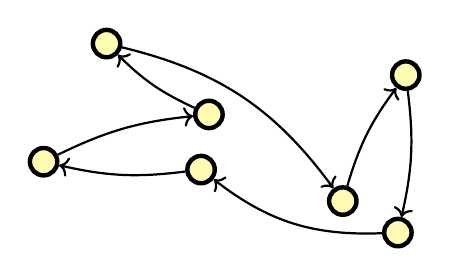
\begin{tikzpicture}[scale=1.00,transform shape]
\node[mynode] at (0.0, 0.0) (pisa) {};
\node[mynode] at (2.0, -0.1) (vinci) {};
\node[mynode] at (3.8, -0.5) (firenze) {};
\node[mynode] at (4.5, -0.9) (rignano) {};
\node[mynode] at (4.6, 1.1) (firenzuola) {};
\node[mynode] at (2.1, 0.6) (serravalle) {};
\node[mynode] at (0.8, 1.5) (castelnuovo) {};

\draw[edgen, thick,->] (firenze) edge[bend left=10] node {} (firenzuola);
\draw[edgen, thick,->] (firenzuola) edge[bend left=10] node {} (rignano);
\draw[edgen, thick,->] (rignano) edge[bend left=20] node {} (vinci);
\draw[edgen, thick,->] (vinci) edge[bend left=10] node {} (pisa);
\draw[edgen, thick,->] (pisa) edge[bend left=10] node {} (serravalle);
\draw[edgen, thick,->] (serravalle) edge[bend left=10] node {} (castelnuovo);
\draw[edgen, thick,->] (castelnuovo) edge[bend left=20] node {} (firenze);
\end{tikzpicture}



\end{document}